\documentclass[]{letter}
\usepackage{graphicx}

\begin{document}

Przykład

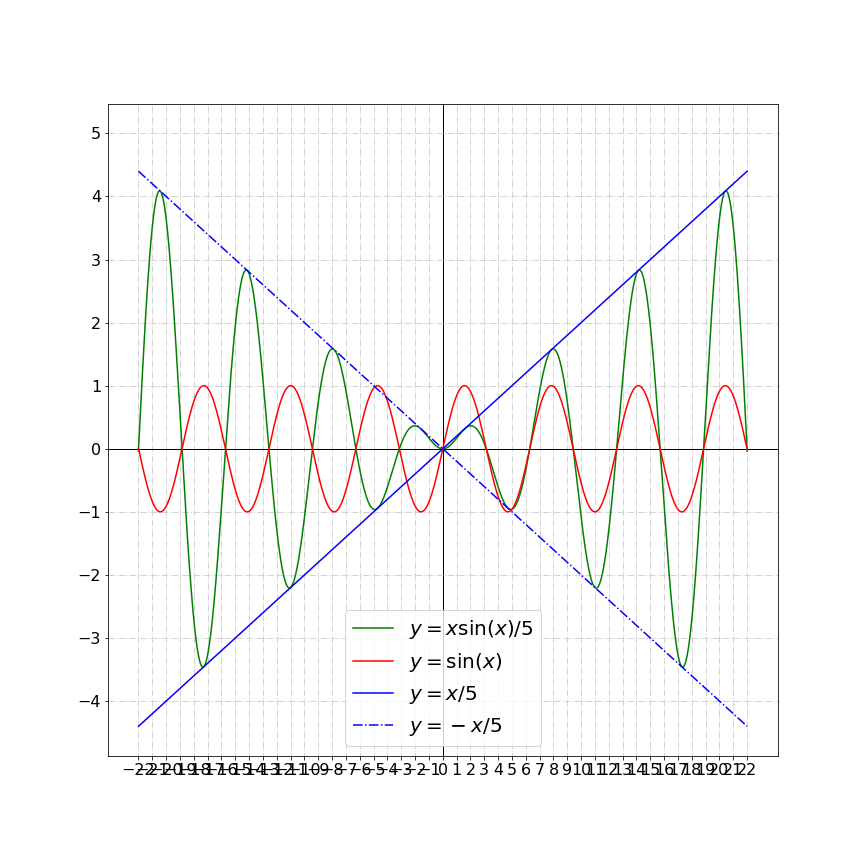
\includegraphics[width=8cm,height=8cm]{pics/graph_mult_1.png}
\newline

Zrobić $\Large y = x\cos(x)$
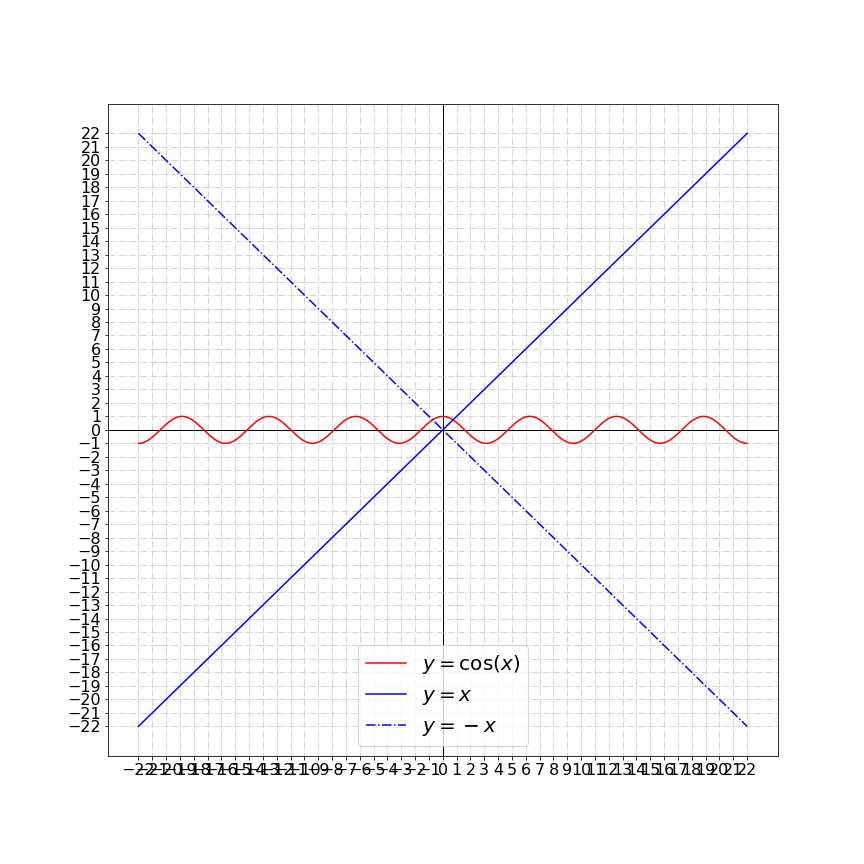
\includegraphics[width=8cm,height=8cm]{pics/graph_mult_2.png}

Przykład
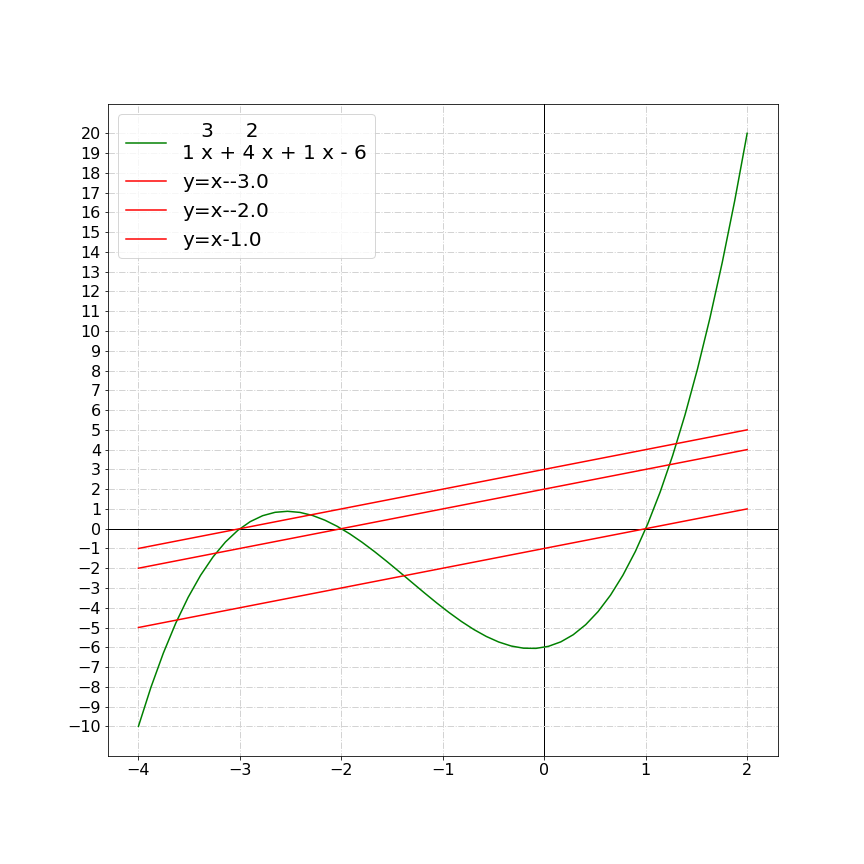
\includegraphics[width=8cm,height=8cm]{pics/graph_mult_3.png}
\newline

Zrobić $\Large y = x(x-2)$
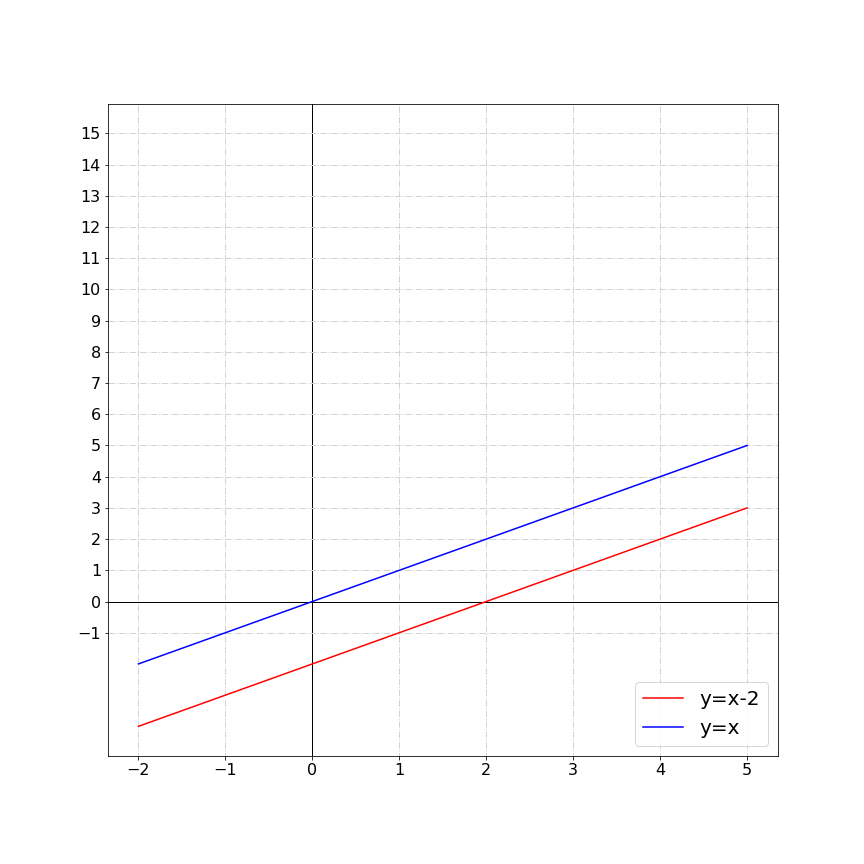
\includegraphics[width=8cm,height=8cm]{pics/graph_mult_4.png}


Przykład
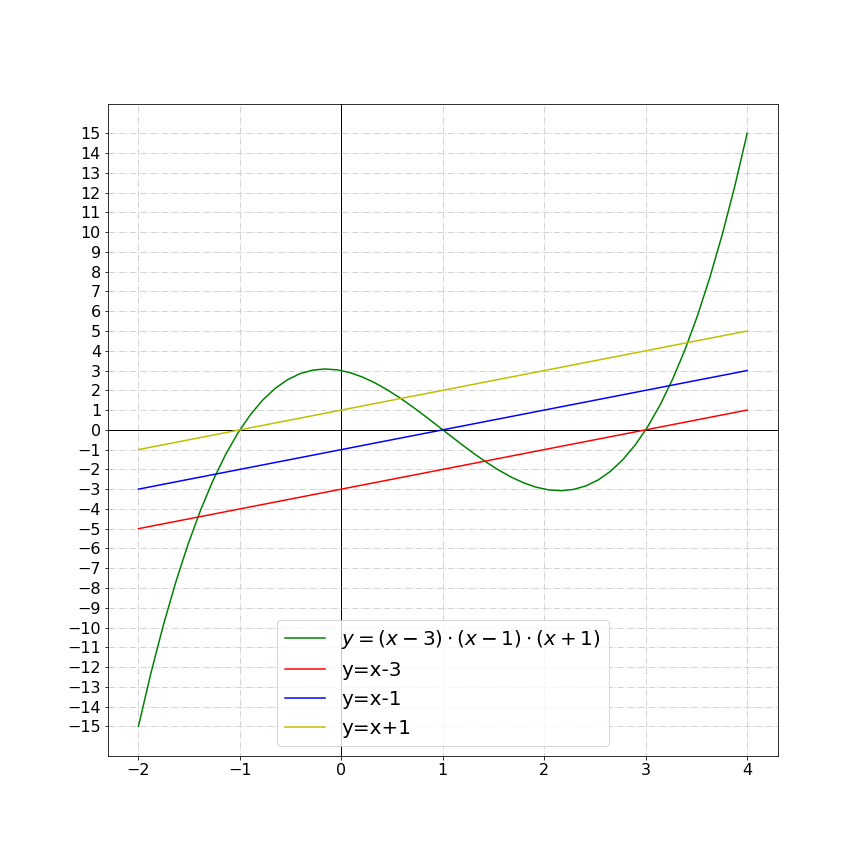
\includegraphics[width=8cm,height=8cm]{pics/graph_mult_5.png}


Zrobić $\Large y = (x+2) x (x-2)$
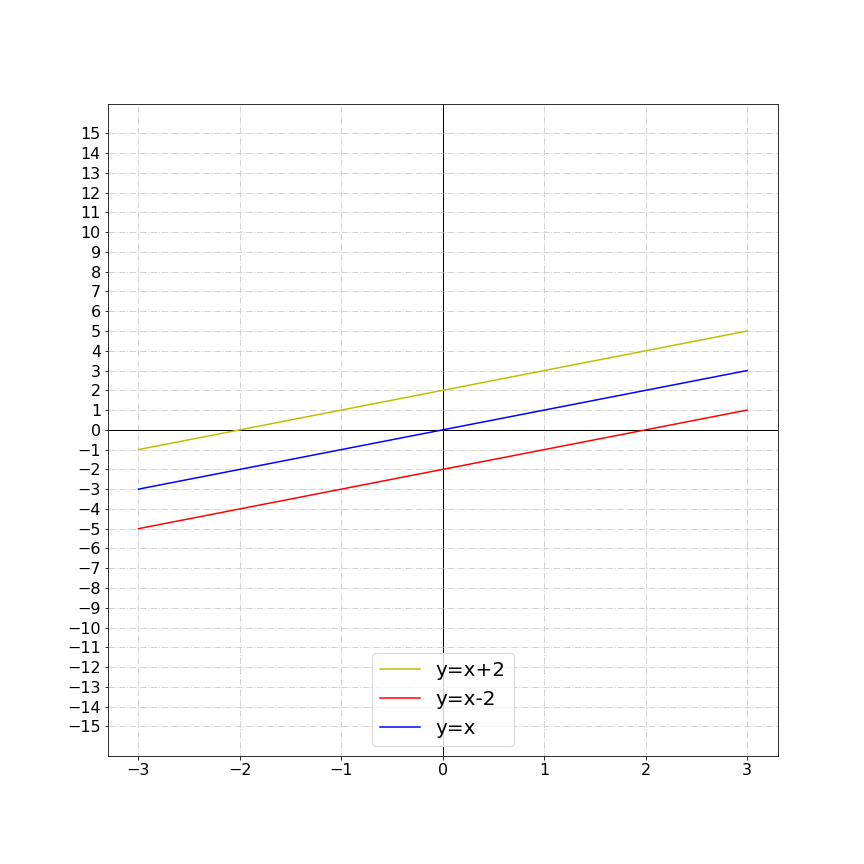
\includegraphics[width=8cm,height=8cm]{pics/graph_mult_6.png}


\end{document}
